\section{Loss function and Gradient Descent} \label{sec:loss_&_gradient_descent}
So far only the concept of what a neural network is was explained, but not how it can learn from data, to understand this it is worth to have first a brief summary of what consists a neural network.

A collection of units having nonlinear activation functions form a layer; layers are stacked from the input to the output with some optional hidden layers in-between; the weighted input of a unit is calculated by multiplying its inputs with some weight parameters and adding a bias term; the unit activation is the output of its activation function applied to the weighted input; and by varying the values of the weights and biases it is possible to reach different model behaviours \textbf{--} this section will only consider the case when the inputs of a unit come from the immediate previous layer and the output is calculated by passing the input values from layer to layer until the last layer (this is called a \textit{feedforward} neural network), other configurations like \acp{ResNet} \cite{resnet2015} and \acp{RNN} also exist, but it is possible to extend the arguments present here to also explain learning in these contexts.

For all neural networks, learning is the process of changing the weights and biases (and possibly other values) in order to produce the desired result. The set of values that are learned during training are called the \textit{parameters} of the network.

The number of parameters gives the degree of freedom that the network has, in a larger parameter space the network has more possible choices and can construct more complex relations. On the other hand, fewer parameters may make it difficult or impossible to represent the full complexity of the data. However, besides requiring more computational power, very complex models break the idea of sparsity and can more easily fall into the problem of overfitting (see \autoref{sub:overfitting}).

The number of parameters in the network is given by its architecture, how many layers it has, how many units in each layer, how the connections are made, and so on. This is a choice made when building the network and is not something that is learned by the algorithm. The set of properties that influence the network but that are not learned are usually called the \textit{hyperparameters}. 

Another example of hyperparameter is the activation functions used in the units, they are chosen when constructing the neural network and can't be learned \textbf{--} however some activations like PReLU have internal learnable parameters \cite{prelu2015}.

Learning is then the process of finding optimal parameters for a network given some hyperparameters. But how can a machine automatically learn the parameters? To do this the network must have some way to quantify the results that it produces, a way to distinguish between good and bad outputs, this is what is called the \textit{loss function}.

Also called the cost or objective, the loss function $J(\bm{x}, \bm{\theta})$ is a function that returns how good the output of the network is, given an input $\bm{x}$ and a set of network parameters $\bm{\theta}$ (represents all trainable parameters: weights, biases, and any others). Learning can then be described as the process of adapting the parameters $\bm{\theta}$ in order to minimize or maximize the objective function (usually minimize, depends on the function used). The choice of function will depend on the type of problem, but two of the most common methods are \gls{MSE} and Categorical Cross Entropy.

\subsection{Mean Squared Error} \label{sub:mse}
This function is the standard squared euclidean distance between two vectors. For a given input $\bm{x}$, the network output $\hat{\bm{y}}$ for this input, and the true desired output $\bm{y}$ (e.g. the corresponding label), the squared distance is calculated as shown in \autoref{eq:squared_distance} \textbf{--} note that the subscript $2$ indicates the euclidean distance (the $\ell_2$ norm).
\begin{equation} \label{eq:squared_distance}
    \| \bm{y} - \hat{\bm{y}} \|_{2}^{2} = \sum_{i}{(y_j - \hat{y_i})^2}
\end{equation}

This distance can also be generalize to matrices or any $n$ dimensional values of $\bm{y}$ by just calculating the element-wise squared differences between $\bm{y}$ and $\hat{\bm{y}}$.

However, simply calculating the distance for one possible input is not good for evaluating how well the network is doing in general. To better evaluate the network's performance it is necessary to see how well it is doing in the entire dataset or some subset of it. For a set $\bm{X}$ of $n$ inputs, the \gls{MSE} is the mean of the squared distances as shown in \autoref{eq:mse}.
\begin{equation} \label{eq:mse}
    J(\bm{X}, \bm{\theta}) = \frac{1}{n}\sum^{n}||\bm{y} - \hat{\bm{y}}||_{2}^{2} = \frac{1}{n}\sum^{n}\sum_{i}{(y_i - \hat{y_i})^2}
\end{equation}

This loss function is usually used for regression problems, where the output can have a range of values and is not simply defined as a $0$ or a $1$. It is also useful to calculate the differences between images in pixel space, like used for autoencoders \cite{autoencoder1991}.


\subsection{Categorical and Binary Cross Entropy} \label{sub:cross_entropy}
Like \gls{MSE} this loss function is calculated by averaging the error over many different inputs, but in this case the error calculated is the cross entropy. Given two discrete probability distributions $\bm{y}$ and $\hat{\bm{y}}$, the cross entropy is calculated as shown in \autoref{eq:cross_entropy}.
\begin{equation}  \label{eq:cross_entropy}
    H(\bm{y}, \hat{\bm{y}}) = -\sum_{i}{y_i\log(\hat{y}_i + \epsilon)}
\end{equation}

The \gls{epsilon} value in this equation is not a part of the cross entropy definition, but when using computers to calculate the logarithm, numbers very close or equal to zero can introduce numerical instabilities. For this reason, in almost all practical implementations it is always added a small constant $\epsilon$ when calculating the cross entropy and other functions that can have similar issues \textbf{--} in Tensorflow \cite{tensorflow2015} the default value for $\epsilon$ is equal to $10^{-7}$.

The cross entropy applied over a set of inputs gives the categorical cross entropy loss as shown in \autoref{eq:categorical_cross_entropy}.
\begin{equation} \label{eq:categorical_cross_entropy}
    J(\bm{X}, \bm{\theta}) = \frac{1}{n}\sum^{n}{ H(\bm{y}, \hat{\bm{y}}) }
\end{equation}

This kind of loss function is useful when dealing with probability distributions, since the concept of entropy is deeply related with information and probability. This makes it a better alternative for classification problems when compared with \gls{MSE}, since the desired output is the class that the input belongs to (one hot encoded) and the network output is a probability distribution over all possible classes. 

But for cases where the output can only assume two values (0 or 1), the categorical cross entropy is reduced to a binary cross entropy. For \acp{GAN}, this is the more useful loss function and it is calculated as shown in \autoref{eq:binary_cross_entropy}.
\begin{equation} \label{eq:binary_cross_entropy}
    J(\bm{X}, \bm{\theta}) = -\frac{1}{n}\sum^{n}\sum_{i}{
        \left( y_i\log(\hat{y_i} + \epsilon) + (1 - y_i) \log(1 - \hat{y_i} + \epsilon) \right)
    }
\end{equation}



\subsection{Minimizing the loss} \label{sub:minimizing_loss}
Having an understanding of what is the loss function, the remaining question is: how can the network use the loss in order to update its parameters? Note that since this function effectively measures how well the network is doing, it can directly be used to guide the parameter changes, the goal is to change the parameters in order to minimize the loss (for now on the goal will only be described as minimization, since it is the most common approach and any maximization problem is equivalent to minimizing the negative of what is being maximized).

Note that the inputs $\bm{x}$ are fixed, given that the dataset is also fixed, and that the goal of using neural networks is that they should learn to model the data and not just choose whatever inputs reduce their loss. So in the eyes of the network $J(\bm{x}, \bm{\theta})$ becomes only $J(\bm{\theta})$. This may seem obvious, but this shows an important intuition that the cost function is a high dimensional surface in $N$ dimensional space, $N$ being the number of parameters of the network. And this demonstrates the importance of having both the network and loss functions be continuous and differentiable functions, since this produces a continuous and differentiable surface that allows for updating the parameters in order to reach a minimum region.

To see how the minimum is reached, it is better to start in a very simplified case where the network has only one parameter $\theta$. Consider a case where the 1-dimensional loss surface assumes the form shown in \autoref{fig:1d_loss}.
\begin{figure}
    \centering
    \caption{Example of a one dimensional loss surface}
    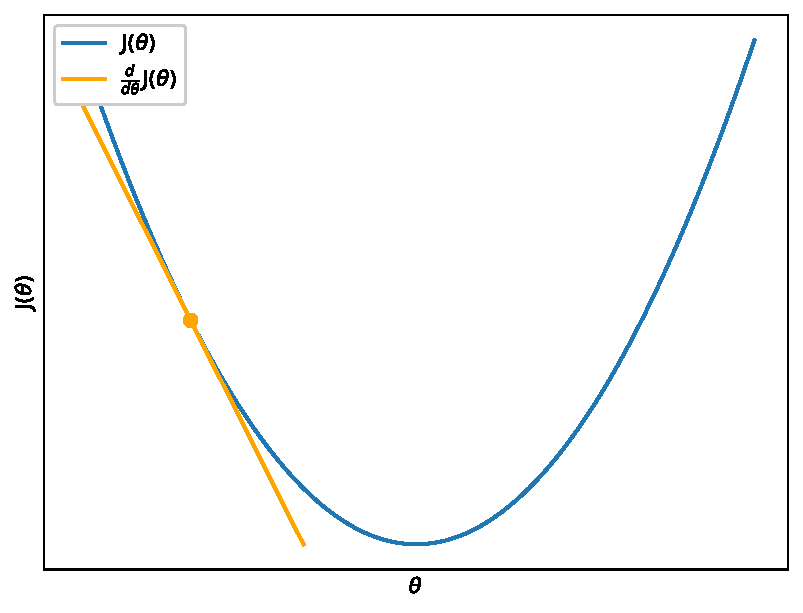
\includegraphics[width=0.5\textwidth]{chapters/NeuralNets/figures/1D-Loss.pdf}
    \fonte{From the author (2021)}
    \label{fig:1d_loss}
\end{figure}

Consider that the network initially starts with the parameter $\theta_0$ and loss $J_0$ at the dot shown in \autoref{fig:1d_loss}. To reduce the loss is to update the parameter $\theta$ in the opposite direction of the surface derivative. This can be shown by the following derivation.
\begin{align}
    J_0 + \Delta J & < J_0 \nonumber \\
    J_0 + \Delta\theta \frac{dJ}{d\theta} & < J_0 \nonumber \\
    \Delta\theta \frac{dJ}{d\theta} & < 0 \nonumber \\
    \sign(\Delta\theta) & = -\sign\left( \frac{dJ}{d\theta} \right) \label{eq:delta_theta_sign}
\end{align}

This derivation above only holds true for small values of $\Delta\theta$, since the derivative is calculated on infinitesimal small values, bigger changes run the risk of overshooting the region where the derivative approximation is reasonable.
\autoref{eq:delta_theta_sign} shows that the parameter change must be in the opposite direction of the change in the loss, the parameter updates can then be written as shown in \autoref{eq:1d_update}.
\begin{equation} \label{eq:1d_update}
    \theta_{i+1} = \theta_{i} + \Delta\theta = \theta_{i} - \eta \frac{dJ}{d\theta}
\end{equation}

\glsunset{learning_rate}
The value \gls{learning_rate} is a positive real number that determines how big are the steps taken when updating the parameters. This value is also a hyperparameter and is called the \textit{learning rate} of the network. A small learning rate is more precise but can make the training very slow, while bigger values are faster, but run the risk of overshooting and zigzaging around the target, or even worse, diverging and never reaching the result. \autoref{fig:1d_weight_update} shows how an initial parameter value is updated when using different values for $\eta$, it can be seen that there is a critical value $\eta_{crit}$ that is able to minimize the loss in a single step, while smaller and bigger values will converge to the minimum in multiple steps, and much bigger values will diverge.
\begin{figure}
    \centering
    \caption{Parameter updates for 1D loss surface in function of learning rate}
    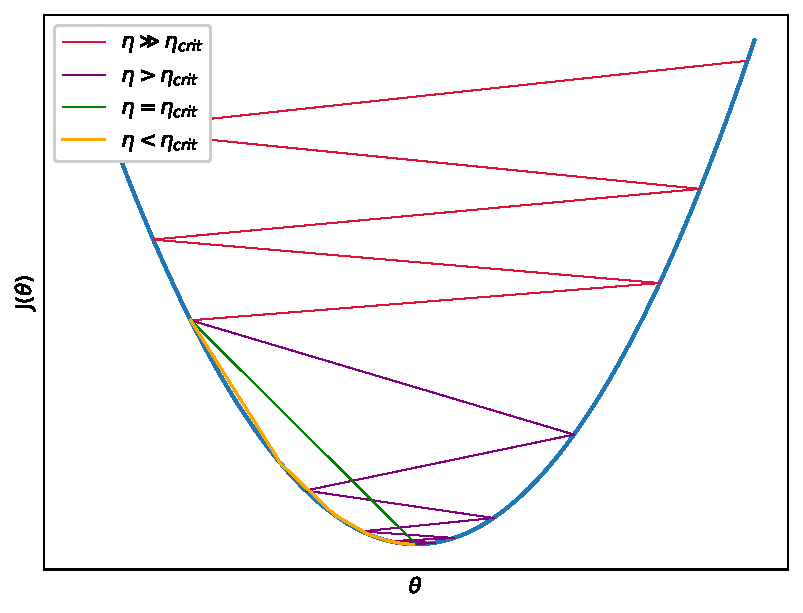
\includegraphics[width=0.5\textwidth]{chapters/NeuralNets/figures/1D-Weight-Update.pdf}
    \fonte{From the author (2021)}
    \label{fig:1d_weight_update}
\end{figure}

For one dimension it is relatively simple to find the critical learning rate, but for very high dimensional problems this is unfeasible or even impossible since a critical value for one parameter is not necessarily the same for all other parameters.

In practice, it is usually necessary to experiment with some values in order to find what best suits the loss surface of the problem, it is also common to employ some sort of dynamic update that slowly reduces the learning rate, allowing for big steps in the beginning while being more precise towards the end.


\subsection{Gradient Descent} \label{sub:gradient_descent}
The same derivation used to obtain \autoref{eq:delta_theta_sign} can be applied to generalize the minimization procedure to higher dimensional parameter spaces, the only difference is to consider the partial derivatives for each parameter. Doing this would reveal that, like in the 1-dimensional case, the change in a parameter $\theta^{(j)}$ must be in the opposite direction of the partial derivative of the loss with respect to this parameter. The parameter update would then be given by \autoref{eq:parameter_update}.
\begin{equation} \label{eq:parameter_update}
    \theta_{i+1}^{(j)} = \theta_{i}^{(j)} - \eta \frac{\partial J}{\partial \theta^{(j)}}
\end{equation}

There is however another way to look at these updates. Recall that the gradient of any scalar function is a vector field composed of all its partial derivatives, so the gradient of the loss function is the vector field given by \autoref{eq:gradient}.
\begin{equation} \label{eq:gradient}
    \renewcommand{\arraystretch}{1.2}
    \nabla_{\bm{\theta}} J = \begin{bmatrix}
        \frac{\partial J}{\partial\theta^{(1)}} \\
        \frac{\partial J}{\partial\theta^{(2)}} \\
        \vdots \\
        \frac{\partial J}{\partial\theta^{(n)}}
    \end{bmatrix}
\end{equation}

Also recall that for any function $f$, its gradient at any given point is a vector that points towards the direction of steepest increase to the function at that point and the negative of this vector points to the steepest decrease \cite[Chapter~4.6]{calculusIII2016}. So the negative of the gradient $\nabla_{\bm{\theta}} J$ gives the direction to update all parameters in order to most reduce the loss function, this is what was being shown element-wise in \autoref{eq:parameter_update}. By grouping the derivatives it is possible to write the parameter updates in a much cleaner way.
\begin{equation} \label{eq:gradient_descent}
    \bm{\theta}_{i+1} = \bm{\theta}_{i} - \eta \nabla_{\bm{\theta}} J(\bm{\theta}_i)
\end{equation}

By repeating the process of calculating the gradient of the loss function and then updating all the network's parameters (given a sufficiently small learning rate), then eventually all parameters will converge to values that minimize the loss function. This is what is referred to as \textit{learning} in a neural network and this iterative process is called \textit{Gradient Descent}, since the steps are taken using the gradient in order to decrease the loss function \textbf{--} for maximization, the only difference is to update in the positive direction of the gradient and this is called \textit{Gradient Ascent}.

One important thing that was left unmentioned is the fact that this algorithm will almost surely converge to a local minimum in the loss surface instead of the global minimum. In the example shown for the 1-dimensional case the surface was very simple, with a single minimum value to converge, but even in these very simple cases it is possible to find surfaces much more complex (e.g. the curve $y = x + 2\sin x$ has infinitely many local minima but no global minimum). For the very high dimensional spaces and very complex geometries of the loss surfaces in neural networks, there will be many valleys where gradient descent will converge, but rarely those will be the optimal solution. The local minimum found will depend on the starting point in parameter space, and there is usually no better to way than just randomly selecting a point\footnote{
    This does not mean that the starting values are picked without any rhyme or reason, the starting point can have a huge impact on the network and it is very important to choose good values. However, initialization techniques are concerned with finding a random distribution with the right values of mean and variance to sample from. The point here is explicitly about the random nature of the starting point and not that this nature has no thought behind it.
}.

So if gradient descent will almost never reach the optimal solution, why would anyone use it? How can someone make sure that the local minimum found is good enough for the problem? Or if someone is trying to build a neural network and the results are not being good, how can this person know if this is caused by a legitimate problem on the network or the dataset, instead of simply being the fact that the training process was unlucky and found a bad local minimum? And perhaps most important, how is it possible that neural networks are achieving so much ground-breaking results while relying on gradient descent to learn?

This is indeed a worry that many researchers in the field have, but there are many options to combat this problem, it can be cited regularization techniques (e.g. $\ell_1$ and $\ell_2$ norms \textbf{--} see \autoref{sub:regularization}) and optimizers (e.g. \glsunset{SGD}\gls{SGD}, momentum, RMSProp, \glsunset{Adam}\gls{Adam} \textbf{--} see \autoref{sub:optimizers}) as examples. 

Besides that, \textcite{lossSurfaces2014} argue that global minimum are not necessarily the best option, since they have a high chance of overfitting to the data (see \autoref{sub:overfitting}), they also empirically verify that for big enough neural networks most local minima are very similar to one another and have high quality. Their conclusion is that in practice it is not worth to strive for the global minimum, given that for large networks local minima have high quality and may even generalize better to unseen data.
